\section{Name Prefix Table}
\label{sec:npt}

\begin{figure}[!h]
  \center
  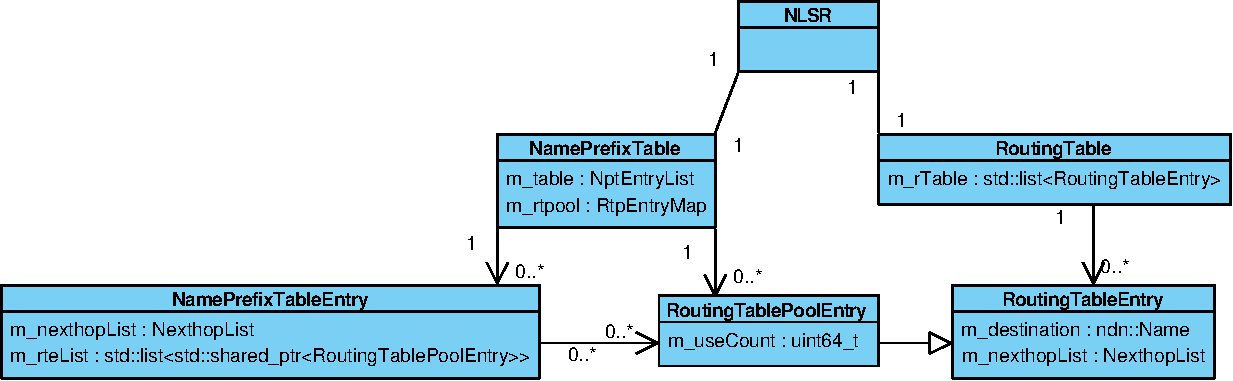
\includegraphics[width=0.8\linewidth]{npt}
  \begin{caption}
    A diagram of the NPT and Routing Table.

    \begin{footnotesize}
      The ``wire'' arrows represent references (i.e. ``x has y''),
      whereas the ``solid'' arrows represent inheritance (i.e. ``y subclasses x''). \\
      The quantification (e.g. 0..*) is standard UML.
    \end{footnotesize}
  \end{caption}
  \label{fig:npt-class-diagram}
\end{figure}

The Name Prefix Table (NPT) is used by NLSR to maintain a list of all known name prefixes advertised by other routers, including router names.
The NPT maintains a collection of NPT entries, where each entry represents a name prefix and all of its associated routing table entries.
Additionally, to optimize the storage and association of the routing table entries, the NPT also maintains a collection of duplicated routing table entries, called routing table pool entries, which have an additional use count attribute.
The NPT entries keep shared pointers to the appropriate routing table pool entries.
If a name prefix is advertised by multiple routers, the name prefix will be represented by only one Name Prefix Table Entry, but will have multiple routing table pool entries  which correspond with each origin router.

If a Name LSA exists with an advertised name prefix, that advertised name prefix must be represented in the NPT.
Thus, if two routers advertise the same name prefix and one Name LSA expires, the NPT entry must not be removed due to the existence of the Name LSA from the other router.

If an any type of LSA for a remote router exists in the LSDB, the remote router's name prefix must be present in the NPT.
An NPT Entry for a router name can be safely removed when there are no more LSAs in the LSDB from the origin router or there are no routing table entries for the origin router.

\subsection{Adding an NPT Entry}
\label{sec:npt-add}
The \texttt{NamePrefixTable::addEntry()} method is the public interface for name prefixes to be added to the NPT.
The name prefix as well as the router's prefix which originates the name prefix are passed as parameters to the interface.
The NPT will look through its collection of routing table pool entries first to see if it already has the appropriate route.
If the NPT locates a local entry, it will increment that entry's use count.
If none can be found, if will check in the Routing Table to see if a ``raw'' routing table entry matching the origin of the prefix is available there.
If one is found, it will create a routing table pool entry with the same information, and a use count of one. This new routing table pool entry will then be used.
If one is not found, a routing table pool entry with no routing information and a use count of one is made, and the NPT entry will retain this ``dummy'' routing information until the Routing Table performs a calculation and updates it.

The rest of the method determines if this NPT entry already exists in the NPT itself.
If it has not been added, i.e. it is new, a new NPT entry will be made and installed in the NPT.
Then the routing table pool entry with the routing information to the origin router's prefix will be added to this new NPT entry.
If the entry already exists in the NPT, then the existing entry will be updated in the same way as the new one.
If the updated NPT entry has next hops, the NPT will update the FIB with the prefix and its next hops.
If there are no next hops, then this means that there is no way for the router to reach the origin.
The FIB entry will be removed, but the NPT entry will be retained, as the routing table may calculate a new route.

\subsection{Removing an NPT Entry}
\label{sec:npt-del}
The \texttt{NamePrefixTable::removeEntry()} method is the public interface for name prefixes to be removed from the NPT.
The name prefix as well as the router's prefix which originates the name prefix are passed as parameters to the interface.
The NPT will use the origin router's name to look through its local collection of routing table pool entries.
Because this is the NPT's centralized, total pool of routing information, if the entry does not exist here it cannot exist in any NPT entries.
In that case, the method ends.
Else, the method will look through the collection of NPT entries for the entry matching the name prefix in the parameters.
If it does not find it, there is nothing to be done, and the method ends.
If it does find a matching entry, it will remove from that entry the routing table pool entry with the origin router prefix matching the one given in the parameters.
The next hop information of the entry is rebuilt, and then the method checks if the entry has any next hops.
If it does, the method will inform the FIB of the change with the name prefix and the next hops.
If the entry no longer has any next hops, this means that there is no routing information to any router advertising that prefix.
In this case, the NPT will remove that entry, as it is no longer useful.

\subsection{Updating an NPT Entry with New Routing Table Entries}
\label{sec:npt-update-with-new-route}
When the Routing Table module has finished calculating, it will notify the NPT using the \texttt{NamePrefixTable::updateWithNewRoute()} interface.
The NPT will then iterate over each of its entries and each entry's routing table pool entry list.
For each routing entry in the list, the NPT will attempt to fetch the new next hop list from the Routing Table, and set the entry's next hop list to that.
If no list is available, it clears the routing table pool entry's next hop list.
Then, \texttt{NamePrefixTable::addEntry()} is called with the current NPT entry and routing table pool entry pair.

\subsection{Adding routing table pool entries to the pool}
\label{sec:npt-rtpe-add}
Whenever a routing table pool entry (RTPE) needs to be constructed, the method \texttt{NamePrefixTable::addRtpeToPool()} is called.
It constructs and inserts into the hash map a pair object whose first element is the origin router prefix, and whose second element is a shared pointer to the actual routing table pool entry object.
As stated in the \texttt{NamePrefixTable::addEntry()} method, the RTPE will have a use count of one.

\subsection{Removing routing table pool entries from the pool}
\label{sec:npt-rtpe-del}
After an RTPE is removed from an NPT entry, it will be deleted from the pool if \texttt{NamePrefixTable::removeEntry()} determines that the RTPE now has a use count of 0.
It will then call \texttt{NamePrefixTable::deleteRtpeFromPool()}, passing the RTPE as a parameter.
The method will erase the element from the hash map that they are contained in.
